\documentclass{bmcart}

%%%%%%%%%%%%%%%%%%%%%%%%%%%%%%%%%%%%%%%%%%%%%%
%%                                          %%
%% CARGA DE PAQUETES DE LATEX               %%
%%                                          %%
%%%%%%%%%%%%%%%%%%%%%%%%%%%%%%%%%%%%%%%%%%%%%%

%%% Load packages
\usepackage{amsthm,amsmath}
\usepackage{graphicx}
%\RequirePackage[numbers]{natbib}
%\RequirePackage{hyperref}
\usepackage[utf8]{inputenc} %unicode support
%\usepackage[applemac]{inputenc} %applemac support if unicode package fails
%\usepackage[latin1]{inputenc} %UNIX support if unicode package fails


%%%%%%%%%%%%%%%%%%%%%%%%%%%%%%%%%%%%%%%%%%%%%%
%%                                          %%
%% COMIENZO DEL DOCUMENTO                   %%
%%                                          %%
%%%%%%%%%%%%%%%%%%%%%%%%%%%%%%%%%%%%%%%%%%%%%%

\begin{document}

	\begin{frontmatter}
	
		\begin{fmbox}
			\dochead{Artículo de investigación}
\setattribute{authorinfo}{text}{}
			
			%%%%%%%%%%%%%%%%%%%%%%%%%%%%%%%%%%%%%%%%%%%%%%
			%% INTRODUCIR TITULO PROYECTO               %%
			%%%%%%%%%%%%%%%%%%%%%%%%%%%%%%%%%%%%%%%%%%%%%%
			
			\title{Red de genes asociados a la alteración de la N-glicosilación de proteínas (HP:0012347)}
			
			%%%%%%%%%%%%%%%%%%%%%%%%%%%%%%%%%%%%%%%%%%%%%%
			%% AUTORES. METER UNA ENTRADA AUTHOR        %%
			%% POR PERSONA                              %%
			%%%%%%%%%%%%%%%%%%%%%%%%%%%%%%%%%%%%%%%%%%%%%%
			
			\author[addressref={aff1}]{\inits{M.P.}\fnm{Mario~}\snm{Perales Díaz}}
			\author[addressref={aff1}]{\inits{E.A.}\fnm{Estela~}\snm{Anaya}}
			\author[addressref={aff1}]{\inits{M.A.R.C.}\fnm{Miguel Ángel~}\snm{Ramírez Corbacho}}
			\author[addressref={aff1}]{\inits{M.L.O.}\fnm{Marcos~}\snm{Llopis Ontañón}}
			
			%%%%%%%%%%%%%%%%%%%%%%%%%%%%%%%%%%%%%%%%%%%%%%
			%% AFILIACION. NO TOCAR                     %%
			%%%%%%%%%%%%%%%%%%%%%%%%%%%%%%%%%%%%%%%%%%%%%%
			
			\address[id=aff1]{%                           % unique id
			  \orgdiv{ETSI Informática},             % department, if any
			  \orgname{Universidad de Málaga},          % university, etc
			  \city{Málaga},                              % city
			  \cny{España}                                    % country
			}
		
		\end{fmbox}% comment this for two column layout
		
		\begin{abstractbox}
			\begin{abstract}
			
			 Se analizaron los genes asociados al fenotipo HP:0012347, correspondiente a una alteración de la N-glicosilación de proteínas.
             A partir de 50 genes anotados en Human Phenotype Ontology, se construyó una red de asociaciones funcionales mediante STRING v12.5, utilizando un umbral de confianza de 800. La red resultante estuvo formada por 41 nodos y 106 aristas,
             distribuidos en tres componentes conexas. El algoritmo de Louvain identificó siete comunidades, cuya caracterización funcional mediante Gene Ontology mostró asociaciones con procesos de N-glicosilación, biosíntesis de glicoproteínas y transporte intracelular.
			 El análisis topológico reveló una densidad de 0.1293, una transitividad de 0.6263 y una distribución heterogénea del grado, con un coeficiente de variación del 53.30\%.
			 Los genes ALG1 y ALG3 presentaron la mayor
			 conectividad, mientras que ALG2 destacó por su
			 centralidad de intermediación y su condición
			 de punto de articulación. MPI presentó el
			 mayor coeficiente de participación entre comunidades.
			 En conjunto, la combinación de análisis funcionales y topológicos permitió identificar diferentes
			 perfiles de relevancia estructural entre las proteínas asociadas al fenotipo.

			\end{abstract}
			\begin{keyword}
				\kwd{N-glicosilación}
				\kwd{Human Phenotype Ontology}
				\kwd{STRING}
				\kwd{red de interacción}
				\kwd{enriquecimiento funcional}
			\end{keyword}
		\end{abstractbox}
	
	\end{frontmatter}
	
	%%%%%%%%%%%%%%%%%%%%%%%%%%%%%%%%%%%%%%%%%%%%%%%%%%%%%%%%%%%%%%%%%%%%%%%%%%%%%%%%%%%%%%%%
	%% EJEMPLO DE LATEX %%                                                                %%
	%% BORRAR ANTES DE ENTREGAR!!!!!!!!!!!!!!!!!!!!!!!!!!!!!!!!!!!!!!!!!!!!!              %%
	%%%%%%%%%%%%%%%%%%%%%%%%%%%%%%%%%%%%%%%%%%%%%%%%%%%%%%%%%%%%%%%%%%%%%%%%%%%%%%%%%%%%%%%%
	
	\section{Introducción}

La glicosilación de proteínas es uno de los procesos celulares que permiten que muchas proteínas puedan desarrollar correctamente sus funciones. Consiste en la incorporación de cadenas de azúcares, denominadas glicanos, a determinadas proteínas durante su formación y procesamiento. Aunque estas modificaciones no siempre son visibles cuando estudiamos una proteína, tienen una gran importancia, ya que pueden influir en su plegamiento, estabilidad, localización y actividad dentro de la célula.

Existen diferentes tipos de glicosilación, pero en este trabajo nos centramos en la N-glicosilación. Este proceso consiste en la unión de glicanos al átomo de nitrógeno de determinados residuos de asparagina presentes en las proteínas. Comienza en el retículo endoplasmático, donde se incorpora inicialmente el glicano, y continúa en el aparato de Golgi, donde puede experimentar distintas modificaciones hasta alcanzar su estructura final.

La importancia de este mecanismo se entiende mejor si tenemos en cuenta que numerosas proteínas necesitan una glicosilación adecuada para mantener su estructura y desempeñar su función. Por tanto, cuando se produce alguna alteración en las etapas de este proceso, pueden aparecer proteínas que no se pliegan correctamente, que presentan problemas de estabilidad o que no llegan al lugar donde deberían actuar. Estas alteraciones pueden tener consecuencias en diferentes procesos celulares y, en determinados casos, estar relacionadas con enfermedades genéticas.

En este contexto, nuestro trabajo se centra en el fenotipo HP:0012347, denominado \textit{Abnormal protein N-linked glycosylation}, que podemos traducir como alteración de la N-glicosilación de proteínas. Este fenotipo se encuentra recogido en Human Phenotype Ontology (HPO) \cite{Kohler2021}, un recurso que permite describir de manera estandarizada las características fenotípicas asociadas a distintas enfermedades.

La elección de este fenotipo nos permite estudiar un proceso biológico concreto y, al mismo tiempo, investigar los genes que pueden estar relacionados con sus alteraciones. En lugar de analizar cada gen de forma independiente, nos interesa conocer cómo se relacionan entre ellos y si participan en mecanismos celulares comunes.

\subsection{Enfermedades asociadas al fenotipo}

Las alteraciones de la N-glicosilación  \cite{Peanne2018} están relacionadas con diferentes enfermedades genéticas, entre las que destacan los trastornos congénitos de la glicosilación, conocidos como CDG por sus siglas en inglés (\textit{Congenital Disorders of Glycosylation}). Estos trastornos se producen como consecuencia de alteraciones genéticas que afectan a distintas etapas de la glicosilación.

Una característica importante de estas enfermedades es su diversidad clínica. Aunque comparten alteraciones en procesos relacionados con la glicosilación, sus manifestaciones pueden ser diferentes dependiendo de los genes afectados y de la función que desempeñen. Esto se debe a que la glicosilación interviene en numerosos procesos celulares y resulta necesaria para el funcionamiento de distintos tejidos y órganos.

Al consultar las asociaciones recogidas en HPO para el término HP:0012347, encontramos varias enfermedades relacionadas con este fenotipo. Entre ellas se encuentran COG5-CDG (ORPHA:263487), el trastorno congénito de la glicosilación de tipo Iu (OMIM:615042), el tipo IId (OMIM:607091), el tipo IIb (OMIM:620546) y el tipo IIm (OMIM:300896).

También aparecen otras enfermedades, como el síndrome de piel arrugada (\textit{Wrinkly skin syndrome}, ORPHA:2834), además de determinados trastornos del neurodesarrollo. Esto pone de manifiesto que las alteraciones de la N-glicosilación no se limitan a una única enfermedad, sino que pueden formar parte de distintos cuadros clínicos.

Es importante señalar que la asociación de una enfermedad con este fenotipo no significa necesariamente que todas las personas afectadas presenten las mismas manifestaciones. HPO recoge relaciones entre características fenotípicas y enfermedades, lo que permite estudiar qué alteraciones pueden compartir distintos trastornos.

Por este motivo, resulta especialmente interesante analizar los genes asociados a HP:0012347. Aunque puedan estar relacionados con enfermedades diferentes, algunos de estos genes participan en procesos biológicos comunes. Estudiar sus relaciones puede ayudarnos a comprender mejor qué mecanismos celulares se encuentran implicados en las alteraciones de la N-glicosilación.

\subsection{Objetivo del trabajo}

El objetivo principal de este trabajo es estudiar los genes asociados al fenotipo HP:0012347 y analizar las relaciones existentes entre ellos para comprender mejor los procesos biológicos implicados en la N-glicosilación de proteínas.

Para comenzar, utilizamos Human Phenotype Ontology (HPO), que nos permite identificar los genes asociados al fenotipo seleccionado. A partir de esta información,empleamos STRING  \cite{Szklarczyk2023}, una base de datos que recoge asociaciones funcionales e interacciones entre proteínas, para construir una red que represente las relaciones entre los productos de estos genes.

La construcción de esta red nos permite pasar de una lista de genes a una representación conjunta de sus posibles relaciones. En ella, los nodos representan proteínas y las conexiones indican asociaciones entre ellas. De esta manera, podemos observar qué proteínas se encuentran más relacionadas y cómo se organiza la red en su conjunto.

Una vez obtenida la red, estudiamos algunas de sus propiedades, como el número de nodos y conexiones, la densidad y otras medidas que permiten describir su estructura. También analizamos la presencia de grupos o comunidades de proteínas mediante técnicas de clustering. Estos grupos pueden ayudarnos a identificar conjuntos de genes que mantienen relaciones especialmente estrechas dentro de la red.

Por último, realizamos un análisis de enriquecimiento funcional, cuyo propósito es identificar procesos biológicos que aparecen representados entre los genes estudiados con mayor frecuencia de la esperada según el conjunto de referencia utilizado. Este análisis nos permite interpretar los resultados desde un punto de vista biológico y relacionar los grupos identificados con funciones celulares concretas.

En conjunto, mediante este procedimiento buscamos comprender cómo se relacionan los genes asociados a las alteraciones de la N-glicosilación y qué funciones biológicas pueden compartir. Así, el análisis de redes nos ofrece una visión más amplia del fenotipo estudiado y nos ayuda a interpretar su relación con diferentes enfermedades genéticas.

	\section{Materiales y métodos}

Descargamos la lista de genes asociados a HP:0012347 desde la API de Human Phenotype Ontology y eliminamos espacios sobrantes y filas sin símbolo génico. Mapeamos los 50 genes a identificadores de STRING para Homo sapiens (taxón 9606), versión 12.5, con una puntuación mínima de 800. Construimos una red no dirigida con las asociaciones que superaron ese umbral y eliminamos aristas duplicadas y bucles.

Calculamos el número de nodos y aristas, el grado medio, la densidad, la transitividad global y las componentes conexas con el paquete \textit{igraph}. Identificamos comunidades mediante el algoritmo de Louvain usando la semilla 123. Para la interpretación funcional, realizamos análisis de sobrerrepresentación de términos de procesos biológicos de Gene Ontology con \textit{clusterProfiler}. Aplicamos la corrección de Benjamini-Hochberg y consideramos significativos los términos con p ajustado inferior a 0,05. En el análisis global usamos como fondo los genes humanos anotados en GO; en el análisis por comunidad usamos los genes de la red como fondo.


\subsection{Análisis topológico y dispersión del grado}

Con el objetivo de caracterizar la organización
estructural de la red de asociaciones proteicas
del fenotipo HP:0012347, se realizó un análisis
topológico mediante el paquete \texttt{igraph}
del lenguaje de programación R.

La red se construyó utilizando STRING v12.5,
considerando un umbral de confianza de 800.

Se calcularon el número de nodos y aristas,
el grado medio, la densidad y la transitividad
global de la red.

Para estudiar la heterogeneidad de la
conectividad de los nodos, se calculó la
distribución del grado, incluyendo la media,
mediana, varianza, desviación típica,
cuartiles y coeficiente de variación.

El coeficiente de variación se calculó como:

\begin{equation}
CV = \frac{s_k}{\bar{k}} \times 100
\end{equation}

donde $s_k$ representa la desviación típica
del grado y $\bar{k}$ su valor medio.

Finalmente, las proteínas se ordenaron según
su grado para identificar aquellas con un
mayor número de asociaciones directas.
	
\section{Resultados}

El término HPO HP:0012347, \textit{Abnormal protein N-linked glycosylation} (alteración de la N-glicosilación de proteínas), está asociado a 50 genes. Los 50 genes se mapearon en STRING \cite{Szklarczyk2023} (versión 12.5, taxón 9606). Con un umbral de puntuación de 800, 41 genes formaron una red con 106 aristas; los 9 genes restantes no tuvieron interacciones que superaran ese umbral. La red presentó una transitividad global de 0.6263 y quedó dividida en 3 componentes conexas.

\subsection{Clustering de la red}
Aplicamos el algoritmo de Louvain \cite{Blondel2008} (semilla 123) a la red de 41 nodos, que la dividió en 7 clusters (Figura~\ref{fig:clusters} y Tabla~\ref{tab:clusters}). Cuatro de ellos tienen al menos 5 genes. El cluster 1 (11 genes) reúne a \textit{ALG1}, \textit{ALG2}, \textit{ALG3}, \textit{ALG6}, \textit{ALG8}, \textit{ALG9}, \textit{ALG11}, \textit{ALG12}, \textit{ALG13}, \textit{PMM2} y \textit{RFT1}. El cluster 2 (8 genes) contiene \textit{DPAGT1}, \textit{DHRSX}, \textit{DOLK}, \textit{DPM1}, \textit{DPM2}, \textit{DPM3}, \textit{MPDU1} y \textit{SRD5A3}. El cluster 3 (6 genes) está formado por \textit{ATP6AP1}, \textit{ATP6AP2}, \textit{ATP6V0A2}, \textit{ATP6V1A}, \textit{ATP6V1E1} y \textit{VMA12}, y el cluster 4 (7 genes) por \textit{COG1} y \textit{COG3} a \textit{COG8}. Los tres clusters restantes son pequeños: \textit{GET4} y \textit{CAMLG} (2 genes), \textit{MPI}, \textit{PGM1} y \textit{PGM2L1} (3 genes), y \textit{DDOST}, \textit{EDEM3}, \textit{MAGT1} y \textit{SSR4} (4 genes).

\begin{figure}[htbp]
	\centering
	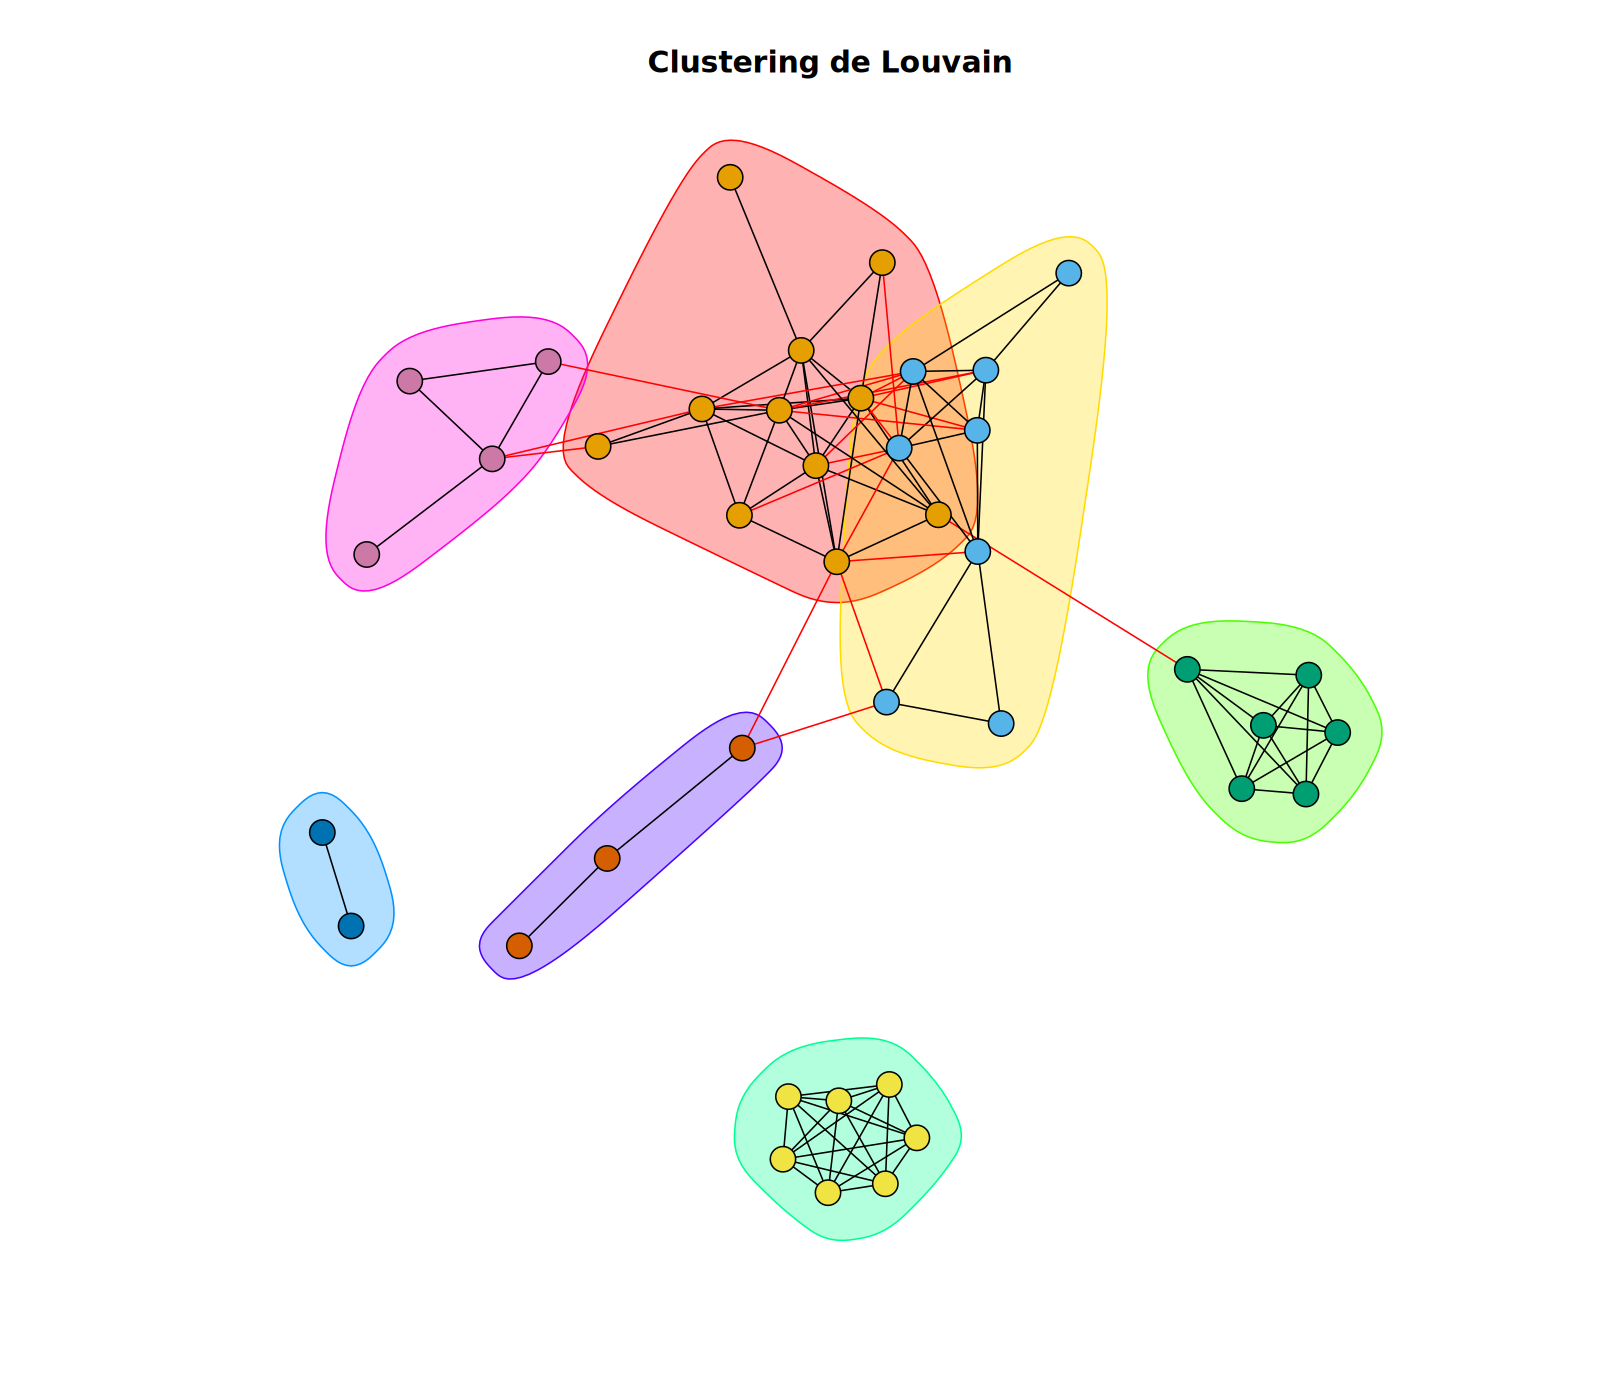
\includegraphics[width=0.9\textwidth]{figures/red_clusters.png}
	\caption{Red de interacciones de STRING (puntuación $\geq$ 800) entre los genes asociados al HP:0012347, coloreada según los clusters de Louvain.}
	\label{fig:clusters}
\end{figure}

\subsection{Enriquecimiento funcional}
Realizamos un análisis de sobrerrepresentación (ORA) de términos de Gene Ontology (procesos biológicos) con \textit{clusterProfiler} \cite{Yu2012}, usando la corrección de Benjamini-Hochberg \cite{BenjaminiHochberg1995} y un umbral de p-valor ajustado de 0,05. Para los 50 genes del HPO, con todos los genes humanos anotados como fondo, obtuvimos 79 términos enriquecidos. Los más significativos fueron \textit{protein N-linked glycosylation} (22 de 50 genes; p ajustado $3{,}2\times10^{-37}$), \textit{glycoprotein metabolic process} (27/50; $3{,}6\times10^{-31}$), \textit{dolichol-linked oligosaccharide biosynthetic process} (14/50; $4{,}6\times10^{-31}$) y \textit{glycoprotein biosynthetic process} (25/50; $5{,}1\times10^{-30}$). También apareció \textit{intra-Golgi vesicle-mediated transport} (7/50; $2{,}4\times10^{-10}$).

Para cada cluster de al menos 5 genes repetimos el análisis tomando como fondo los 41 genes de la red (Tabla~\ref{tab:clusters}). El cluster 1 se enriqueció en \textit{protein N-linked glycosylation} (11/11) y en \textit{dolichol-linked oligosaccharide biosynthetic process} (10/11). El cluster 4 se enriqueció en términos de transporte y localización de proteínas, como \textit{intracellular protein localization} y \textit{vesicle-mediated transport} (7/7). El cluster 2 solo mostró términos genéricos de metabolismo de fosfato (6/8), y el cluster 3 un único término muy general, \textit{biological regulation} (6/6).

\begin{table}[htbp]
	\caption{Clusters de Louvain con al menos 5 genes y término GO más significativo de cada uno.}
	\label{tab:clusters}
	\begin{tabular}{rrp{6cm}r}
		\hline
		Cluster & Genes & Término GO principal & p ajustado \\
		\hline
		1 & 11 & protein N-linked glycosylation & $9{,}8\times10^{-5}$ \\
		2 & 8 & phosphorus metabolic process & $7{,}1\times10^{-3}$ \\
		3 & 6 & biological regulation & $2{,}9\times10^{-2}$ \\
		4 & 7 & intracellular protein localization & $1{,}8\times10^{-4}$ \\
		\hline
	\end{tabular}
\end{table}

\subsection{Caracterización topológica y
dispersión de la red}

La red de asociaciones proteicas correspondiente
al fenotipo HP:0012347, construida mediante
STRING v12.5 con un umbral de confianza de 800,
estuvo formada por 41 nodos y 106 aristas,
distribuidos en tres componentes conexas.

La densidad de la red fue de 0.1293 y la
transitividad global de 0.6263.

El grado medio de los nodos fue de 5.1707,
con una mediana de 5 y una desviación típica
de 2.7559. La varianza del grado fue de
7.5951 y el coeficiente de variación alcanzó
el 53.30\%.

El grado mínimo fue de 1 y el máximo de 11.
El primer y tercer cuartil fueron 3 y 6,
respectivamente.

Estos resultados muestran una distribución
heterogénea del número de asociaciones
entre las proteínas analizadas.

\begin{table}[htbp]
\centering
\caption{Medidas topológicas y de dispersión
de la red HP:0012347.}
\label{tab:dispersion_red}

\begin{tabular}{lc}
\hline
Medida & Valor \\
\hline
Nodos & 41 \\
Aristas & 106 \\
Componentes conexas & 3 \\
Densidad & 0.1293 \\
Transitividad & 0.6263 \\
Grado medio & 5.1707 \\
Mediana & 5 \\
Varianza & 7.5951 \\
Desviación típica & 2.7559 \\
Coeficiente de variación & 53.30\% \\
Grado mínimo & 1 \\
Grado máximo & 11 \\
Primer cuartil & 3 \\
Tercer cuartil & 6 \\
\hline
\end{tabular}
\end{table}

\begin{figure}[htbp]
\centering
\includegraphics[width=0.85\textwidth]
{../results/analisis_avanzado/distribucion_grado.pdf}
\caption{Distribución del grado de los nodos de
la red HP:0012347. La línea discontinua
representa el grado medio.}
\label{fig:distribucion_grado}
\end{figure}

\begin{figure}[htbp]
\centering
\includegraphics[width=0.75\textwidth]
{../results/analisis_avanzado/boxplot_grado.pdf}
\caption{Diagrama de cajas de la distribución
del grado de los nodos de la red.}
\label{fig:boxplot_grado}
\end{figure}

\subsubsection{Identificación de proteínas con mayor conectividad}

El análisis del grado permitió identificar las proteínas
con mayor número de asociaciones directas dentro de la
red. Como se observa en la Figura~\ref{fig:top10_grado},
los genes \textit{ALG1} y \textit{ALG3} presentaron el
mayor grado, con 11 conexiones cada uno.

Los genes \textit{ALG6}, \textit{PMM2}, \textit{DPM1}
y \textit{DPAGT1} presentaron 9 conexiones, seguidos
de \textit{ALG12} y \textit{ALG11}, con 8 conexiones,
y \textit{DPM2} y \textit{DOLK}, con 7 conexiones.

Los genes ALG1 y ALG3 presentaron una conectividad
superior al doble del grado medio de la red, lo que
permite identificarlos como candidatos a hubs.

\begin{figure}[htbp]
    \centering
    \includegraphics[width=0.85\textwidth]
    {../results/analisis_avanzado/top10_grado.pdf}
    \caption{Diez proteínas con mayor grado en la red
    de asociaciones proteicas del fenotipo HP:0012347.}
    \label{fig:top10_grado}
\end{figure}



\subsection{Análisis de centralidades y proteínas puente}

El análisis de centralidades permitió identificar
proteínas relevantes según diferentes criterios
estructurales, más allá del número de asociaciones
directas.

Los genes \textit{ALG1} y \textit{ALG3} destacaron
en varias medidas de centralidad. ALG1 presentó los
mayores valores de centralidad armónica (0.4813),
cercanía (0.5000) y autovector (1.0000), mientras
que ALG3 obtuvo el mayor valor de PageRank (0.0447).

Sin embargo, el mayor valor de intermediación
correspondió a \textit{ALG2} (0.1960), seguido
de \textit{ATP6V0A2} (0.1667) y \textit{PMM2}
(0.1518).

\begin{table}[htbp]
\centering
\caption{Genes con mayor puntuación en cada medida
de centralidad y conectividad entre comunidades.}
\label{tab:centralidades_maximas}
\begin{tabular}{lcr}
\hline
Medida & Gen & Valor \\
\hline
Grado & ALG1, ALG3 & 11 \\
Intermediación & ALG2 & 0.1960 \\
Armónica & ALG1 & 0.4813 \\
Cercanía & ALG1 & 0.5000 \\
Autovector & ALG1 & 1.0000 \\
PageRank & ALG3 & 0.0447 \\
Participación & MPI & 0.6667 \\
Conexiones externas & DPAGT1 & 5 \\
\hline
\end{tabular}
\end{table}

\subsubsection{Conectividad entre comunidades}

El mayor coeficiente de participación correspondió
al gen \textit{MPI} (0.6667), seguido de
\textit{SRD5A3} (0.6250) y \textit{PMM2} (0.5679).

Por otro lado, \textit{DPAGT1} presentó el mayor
número de conexiones externas, con cinco asociaciones
con proteínas pertenecientes a otras comunidades.

La modularidad de la partición de Louvain fue de
0.5688.

Se identificaron seis puntos de articulación:
\textit{ALG11}, \textit{ATP6V0A2}, \textit{ALG2},
\textit{DDOST}, \textit{PGM2L1} y \textit{MPI}.

La eliminación individual de cualquiera de estos
nodos incrementa el número de componentes conexas
de la red.

\begin{figure}[htbp]
    \centering
    \includegraphics[width=0.95\textwidth]
    {../results/analisis_avanzado/red_intermediacion.pdf}
    \caption{Red coloreada según las comunidades
    de Louvain. El tamaño de los nodos es proporcional
    a su centralidad de intermediación. Los bordes
    rojos identifican los puntos de articulación.}
    \label{fig:red_intermediacion}
\end{figure}

\subsubsection{Relación entre las medidas de centralidad}

El análisis de correlación de Spearman mostró una
elevada concordancia entre el grado y PageRank
($\rho=0.906$), así como entre el coeficiente de
participación y las conexiones externas
($\rho=0.964$).

Por el contrario, la correlación entre grado e
intermediación fue moderada ($\rho=0.523$), mientras
que la correlación entre grado y participación
fue de 0.410.

Estos resultados muestran que las medidas analizadas
proporcionan información parcialmente complementaria
sobre la organización estructural de la red.

\begin{figure}[htbp]
    \centering
    \includegraphics[width=0.9\textwidth]
    {../results/analisis_avanzado/correlaciones_centralidad.pdf}
    \caption{Matriz de correlaciones de Spearman
    entre las medidas de centralidad y conectividad
    entre comunidades.}
    \label{fig:correlaciones_centralidad}
\end{figure}

\begin{figure}[htbp]
    \centering
    \includegraphics[width=0.85\textwidth]
    {../results/analisis_avanzado/grado_intermediacion.pdf}
    \caption{Relación entre el grado y la centralidad
    de intermediación de los nodos. Los colores
    representan las comunidades de Louvain.}
    \label{fig:grado_intermediacion}
\end{figure}

	\section{Discusión}

La red de asociaciones proteicas del fenotipo
HP:0012347 presentó una densidad de 0.1293
y una transitividad global de 0.6263.

Estos resultados muestran una conectividad global
limitada junto con una tendencia al agrupamiento
local. Esta organización es compatible con la
existencia de comunidades, identificadas
posteriormente mediante el algoritmo de Louvain.
Los clusters recuperan complejos y rutas conocidos: 
las enzimas \textit{ALG} de la síntesis del oligosacárido ligado
a dolicol, el complejo COG, que participa en el tráfico dentro
del Golgi, y las subunidades de la V-ATPasa. Que los genes más
centrales por centralidad armónica sean \textit{ALG1}, \textit{ALG3}, \textit{ALG6}, 
\textit{PMM2} y \textit{ALG11} es coherente con el papel de esta ruta como paso previo a 
la N-glicosilación.

El enriquecimiento global confirma que el fenotipo está asociado a la glicosilación, 
pero este resultado era esperable, porque los genes se eligieron precisamente por su
relación con ella. Más informativo es el análisis por clusters, que separa la síntesis
del precursor (cluster 1), el metabolismo del dolicol y la manosilación (cluster 2) 
y el tráfico intracelular de proteínas (cluster 4). En cambio, el cluster 3,
formado por subunidades de la V-ATPasa, solo devolvió el término genérico 
\textit{biological regulation}, y el cluster 2 solo términos muy amplios de metabolismo 
del fosfato. Estos resultados no deben sobreinterpretarse, pues la identidad de esos 
clusters se deduce de los genes que los componen y no del enriquecimiento.

El análisis tiene varias limitaciones. Nueve de los 50 genes 
(\textit{B4GALT1}, \textit{SLC35A2}, \textit{UGGT1}, \textit{GORAB}, \textit{MAN2B2},
\textit{MGAT2}, \textit{SLC37A4}, \textit{SLC39A8} y \textit{MAN1B1}) no tienen 
interacciones con puntuación mayor o igual que 800 y quedan fuera de la red y 
de todas las métricas. Bajar el umbral los incorporaría a costa de interacciones 
menos fiables. Además, el algoritmo de Louvain es estocástico, por lo que el número y 
la composición de los clusters pueden variar entre ejecuciones y versiones de 
\textit{igraph}. Por último, el fondo de solo 41 genes reduce la potencia del ORA por 
cluster, y solo 22 de los 50 genes tienen anotado el término 
\textit{protein N-linked glycosylation} en GO, lo que apunta a que las anotaciones de GO 
y de la HPO son incompletas.

\subsection{Organización topológica y heterogeneidad de la red}

El análisis topológico de la red permitió ampliar la
caracterización de los genes asociados al fenotipo
HP:0012347 más allá de la identificación de comunidades
y del enriquecimiento funcional.

La red presentó una densidad del 12.93\% y una
transitividad global de 0.6263. La coexistencia de
una densidad limitada y una transitividad relativamente
elevada sugiere una organización en grupos locales
de proteínas interconectadas, en consonancia con las
comunidades identificadas mediante el algoritmo de Louvain.

El análisis de la distribución del grado mostró una
desviación típica de 2.7559 y un coeficiente de variación
del 53.30\%, lo que refleja una heterogeneidad apreciable
en la conectividad de las proteínas.

Los genes \textit{ALG1} y \textit{ALG3} destacaron
por presentar 11 asociaciones cada uno, superando
el doble del grado medio de la red. Ambos pertenecen
al cluster 1, identificado previamente mediante Louvain,
que presentó un enriquecimiento significativo en
procesos relacionados con la N-glicosilación de proteínas.

Asimismo, otros genes con elevada conectividad,
como \textit{ALG6}, \textit{PMM2}, \textit{DPM1}
y \textit{DPAGT1}, pertenecen a los dos primeros
clusters de la red.

Estos resultados sugieren que las proteínas con mayor
grado se concentran en comunidades relacionadas con
los mecanismos de glicosilación y su metabolismo
asociado.

No obstante, una elevada conectividad en STRING no
implica necesariamente una mayor esencialidad biológica,
relevancia clínica o relación causal con la gravedad
del fenotipo. Por ello, resulta conveniente complementar
el análisis del grado con otras medidas de centralidad
y robustez de la red.


\subsection{Relevancia estructural y conectividad
entre comunidades}

El análisis de centralidades permitió distinguir
diferentes formas de importancia estructural dentro
de la red de asociaciones proteicas.

Aunque ALG1 y ALG3 presentaron el mayor grado,
ALG2 destacó por su centralidad de intermediación
y por constituir un punto de articulación.

Este resultado sugiere que ALG2 desempeña un papel
relevante en la conectividad de la red que no puede
explicarse exclusivamente por el número de
asociaciones directas.

Asimismo, ATP6V0A2 presentó una elevada
intermediación y constituyó otro punto de
articulación, a pesar de no encontrarse entre
los genes con mayor grado.

El análisis de participación permitió identificar
a MPI, SRD5A3 y PMM2 como candidatos relevantes
para estudiar las relaciones entre comunidades.

PMM2 destacó simultáneamente por su conectividad,
intermediación y participación, lo que sugiere
un papel estructural relevante tanto a nivel local
como en la organización global de la red.

La identificación de seis puntos de articulación
pone de manifiesto la existencia de nodos cuya
eliminación puede modificar la conectividad de
la red.

Por otro lado, la correlación moderada entre grado
e intermediación justifica la utilización de
múltiples medidas de centralidad, puesto que
cada una caracteriza diferentes propiedades
estructurales.

No obstante, los resultados deben interpretarse
teniendo en cuenta que STRING representa asociaciones
funcionales y que la selección del umbral de
confianza condiciona la topología obtenida.

La relevancia topológica de una proteína no implica
necesariamente su esencialidad biológica ni permite
establecer directamente relaciones causales con
la gravedad del fenotipo.

Estos hallazgos constituyen una base para evaluar
posteriormente la vulnerabilidad y robustez de la red
mediante simulaciones de eliminación de nodos.

	\section{Conclusiones}

El análisis de HP:0012347 recuperó una red de 41 genes con 106 asociaciones a un umbral STRING de 800; nueve genes de la lista inicial no tuvieron interacciones que superaran ese corte. La red se organizó en siete comunidades de Louvain. El enriquecimiento global y el análisis de las comunidades señalaron procesos relacionados con la N-glicosilación y la biosíntesis de glicoproteínas, así como con el transporte y la localización intracelular de proteínas.

Los resultados dependen del umbral de STRING, de las anotaciones disponibles y del fondo elegido para el enriquecimiento. Por ello, las comunidades y los términos GO se interpretan como patrones de asociación funcional que ayudan a describir los genes, no como prueba de causalidad.

	
	
	%%%%%%%%%%%%%%%%%%%%%%%%%%%%%%%%%%%%%%%%%%%%%%
	%% OTRA INFORMACIÓN                         %%
	%%%%%%%%%%%%%%%%%%%%%%%%%%%%%%%%%%%%%%%%%%%%%%
	
	\begin{backmatter}
	
		\section*{Abreviaciones}
		\begin{description}
			\item[CDG] Trastornos congénitos de la glicosilación (\textit{Congenital Disorders of Glycosylation}).
			\item[GO] Gene Ontology.
			\item[HPO] Human Phenotype Ontology.
			\item[ORA] Análisis de sobrerrepresentación (\textit{Over-Representation Analysis}).
			\item[STRING] Search Tool for the Retrieval of Interacting Genes/Proteins.
		\end{description}

		\section*{Disponibilidad de datos y materiales}
		Los scripts y materiales del proyecto están disponibles en el repositorio del grupo: \texttt{github.com/marcosLlopis/project\_template\_biologia}.

		\section*{Contribución de los autores}
		M.P.D. desarrolló el código reproducible para obtener los genes asociados al término HPO y construir la red. E.A. trabajó el fenotipo, las enfermedades asociadas y la introducción. M.A.R.C. se encargó del análisis de comunidades. M.L.O. coordinó el grupo y desarrolló el análisis topológico avanzado, incluyendo las medidas de dispersión, centralidad y conectividad entre comunidades. Todos los autores son responsables de comprender y defender el trabajo completo.

		\bibliographystyle{bmc-mathphys} % Style BST file (bmc-mathphys, vancouver, spbasic).
		\bibliography{bibliography}      % Bibliography file (usually '*.bib' )
	
	\end{backmatter}
\end{document}
